%
% -- Manlio Modugno

\documentclass{beamer} 
\usepackage{eulervm}
%\usepackage{booktabs}
\usepackage{listings}
\usepackage{bold-extra}
\usepackage{cancel}
\usepackage{fancybox}
\usepackage{soul}
\usepackage[english]{babel}
\usepackage[utf8]{inputenc}
\usepackage{hyperref}
\usepackage{amsmath}
\usepackage{booktabs}
%\hypersetup{colorlinks=true,urlcolor=blue}

\newcommand{\codefont}{\fontsize{6}{8}\selectfont}
\lstset{language=[Sharp]C, 
captionpos=b, 
frame=lines,
lineskip= 1pt, %space between lines
basicstyle=\codefont, 
keywordstyle=\color{blue}, 
commentstyle=\color{green}, 
stringstyle=\color{red}, 
numbers=left, 
numberstyle=\tiny, 
stepnumber=2,
numbersep=5pt,
breaklines=true, 
breakatwhitespace=false,
showstringspaces=false,
frame=single,
tabsize=2,
emph={double,bool,int,unsigned,char,true,false,void},
emphstyle=\color{blue},
emph={Assert,Test},
emphstyle=\color{red},
emph={[2]\using,\#define,\#ifdef,\#endif},
emphstyle={[2]\color{blue}}
}

\mode<presentation>
\definecolor{title_color}{RGB}{2,128,181} 
\usetheme{Ilmenau}
\usecolortheme[named=title_color]{structure}
\setbeamercolor{palette quaternary}{use=structure,fg=black,bg=white} %header footer color
\useoutertheme[subsection=false]{smoothbars}
\setbeamercovered{transparent}
\setbeamertemplate{navigation symbols}{}
\setbeamerfont{subsection in toc}{size=\scriptsize}

\title{Fraud Detection}
\author{Manlio Modugno}
\institute[GMTechnologies] 

\date[]{\today}

\subject{}

\graphicspath{{img/}}
\pgfdeclareimage[height=0.6cm]{mfg-logo}{img/mfgLogo}
\logo{\pgfuseimage{mfg-logo}}


\setbeamertemplate{bibliography entry title}{}
\setbeamertemplate{bibliography entry location}{}
\setbeamertemplate{bibliography entry note}{}

%
% Content start
%
\begin{document}
\begin{frame}
  \titlepage
\end{frame}

\begin{frame}
  \frametitle{Topics}
  \tableofcontents
\end{frame}


\section{Fraud Detection}
\subsection{Intro/Goal}
\begin{frame}
  \frametitle{Intro/Goal}
  \begin{itemize}
	\item<+-> Fraud born with human beings.. and nowadays is a big problem in e-commerce...
	\item<+-> List (some) countermeasures used by industry 
	\item<+-> Understand difference between hash fingerprint and features
   \end{itemize}
\end{frame}


\subsection{How to tackle fraud?}
\begin{frame}
  \frametitle{How to tackle fraud?}
  \begin{itemize}
	\item<+-> \textbf{manual:} (quite) simple when made by humans, really inefficient and error prone
	\item<+-> \textbf{automatic:} complex, efficient and can overwhelm manual fraud detection in quality
	\item<+-> \textbf{automatic} could be \textbf{total} or \textbf{partial}..
	\item<+-> \textbf{total:} a system can totally tackle autonomously fraud problem
	\item<+-> \textbf{partial:} remove all false positive and submit to humans true positives sorted by fraud probability
	\item<+-> \textbf{automatic} sounds good... what we need?
   \end{itemize}
\end{frame}

\subsection{Expert rules}
\begin{frame}
  \frametitle{How to tackle fraud? Expert rules}
  \begin{itemize}
	\item<+-> Incorporate rules in the system from people who knows/has direct experience of a given domain..
	\item<+-> They can work... but they can contradict other custom rules during time... 
		\item<+-> ... and could not be efficient..
   \end{itemize}
\end{frame}


\begin{frame}[containsverbatim]
	\frametitle{custom rule example}
	``People flying to Brazil are fraudsters!''  \\
	\begin{lstlisting}
public class SomeFancyFraudDetectionClass{

	public bool detect(String destination){
		return 	destination.equals("Brazil");
	}
}
	\end{lstlisting}
	Not a good rule... we lose a lot of good people, and all the fraudsters flying to the rest of the world continue to hurt us 
\end{frame}

\begin{frame}[containsverbatim]
	\frametitle{custom rule example}
	``Ok, refine this.. People departing from Italy and flying to Brazil are fraudsters!''  \\
	\begin{lstlisting}
public class SomeFancyFraudDetectionClass{
	public bool detect(String departure, String destination){
		return 	departure.equals("Italy") && destination.equals("Brazil");
	}
}
	\end{lstlisting}
	A little better, but we have still problems.. \\
	
    ``Ok, refine this.. People x and or y and t -t...''  \\
	\begin{lstlisting}
public class SomeFancyFraudDetectionClass{
	public bool detect(String departure, String destination){
        //complex implementation...
	}
}
	\end{lstlisting}
	Could work... but is it the best we can do? Perhaps reducing fraud in this way reduce also earnings because we don't authorize people that can actually buy..  
\end{frame}

\subsection{Machine Learning}
\begin{frame}
  \frametitle{How to tackle fraud? Scientific approach}
  \begin{itemize}
	\item<+-> In addition to (good) Expert Rules, scientific approaches can be used.. 
	\item<+-> Statistic, Operative Research, Machine Learning, Deep Learning, etc.. 
   \end{itemize}
\end{frame}

\begin{frame}
  \frametitle{Machine Learning (Feature)}
  \begin{itemize}
	\item<+-> Supervised / unsupervised learning.. 
	\item<+-> Random Forest, KNN, K-means, SVM, Neural/Bayesan Networks, Deep learning, Logistic regression...
	\item<+-> WTF?!.. a lot exists, they are (quite) complex in \textbf{implementation} and \textbf{evaluation} (Accuracy, Precision, Recall, F-measure...)
	\item<+-> But almost all of them have a common shared point... \underline{FEATURE}
   \end{itemize}
\end{frame}

\subsection{Feature}
\begin{frame}
  \frametitle{What is a feature?}
  \begin{itemize}
	\item<+-> a \textbf{descriptive} feature is an information unit from knowledge base.. age, street, amount,...
	\item<+-> a \textbf{descriptive} feature can be useful or not in respect of a given domain.. for example hair color in marketing vs financial field..
	\item<+-> ...can be extracted from other features... payments time events standard deviation, median, etc.. 
	\item<+-> a \textbf{target} feature is the truth in respect of the associated set of descriptive features (in supervised learning case, aka when we are lucky!..)
   \end{itemize}
\end{frame}

\subsection{Example}
\begin{frame}
  \frametitle{Example\footnotemark}
  \begin{itemize}
	\item<+-> Suppose a financial company wants to predict if a loan will be repaid
	\item<+-> OCCUPATION, AGE and LOAN-SALARY RATIO are descriptive features
	\item<+-> OUTCOME is the target feature	
   \end{itemize}
   \footnotetext[1]{This and subsequent examples are from \cite{KelleherMacNameeDArcy15}}
\end{frame}

\begin{frame}
  \frametitle{Example}
\begin{center}
 \begin{tabular}{c c c c} 
 \hline
 OCCUPATION & AGE & LOAN-SALARY RATIO & OUTCOME \\ [0.5ex] 
 \hline
industrial & 34 & 2.96 & repay \\
professional & 41 & 4.64 & default \\
professional & 36 & 3.22 & default \\
professional & 41 & 3.11 & default \\
industrial & 48 & 3.80 & default \\
industrial & 61 & 2.52 & repay \\
professional & 37 & 1.50 & repay \\
professional & 40 & 1.93 & repay \\
industrial & 33 & 5.25 & default \\
industrial & 32 & 4.15 & default \\
\end{tabular}
\end{center}
\end{frame}

\begin{frame}[containsverbatim]
	\frametitle{prediction model}
	Simple prediction model made by human (could be an Expert Rule) \\
	\begin{lstlisting}
if(LOAN-SALARY RATIO > 3){
  OUTCOME = default;
} else {
  OUTCOME = repay
}
	\end{lstlisting}
\end{frame}

\begin{frame}
  \frametitle{Example}
  What if we have millions of records with hundreds of descriptive features?
\begin{center}
\resizebox{\textwidth}{!}{%
 \begin{tabular}{c c c c c c c c c} 
 \hline
 ID & Amount & Salary & Ratio & Age & Occupation & Property & Type & Outcome \\ [0.5ex] 
 \hline
1 & 245100 & 66400 & 3.69 & 44 & industrial & farm & stb & repay \\
2 & 90600 & 75300 & 1.2 & 41 & industrial & farm & stb & repay \\
3 & 195600 & 52100 & 3.75 & 37 & industrial & farm & ftb & default \\
4 & 157800 & 67600 & 2.33 & 44 & industrial & apartment & ftb & repay \\
5 & 150800 & 35800 & 4.21 & 39 & professional & apartment & stb & default \\
6 & 133000 & 45300 & 2.94 & 29 & industrial & farm & ftb & default \\
7 & 193100 & 73200 & 2.64 & 38 & professional & house & ftb & repay \\
8 & 215000 & 77600 & 2.77 & 17 & professional & farm & ftb & repay \\
9 & 83000 & 62500 & 1.33 & 30 & professional & house & ftb & repay \\
10 & 186100 & 49200 & 3.78 & 30 & industrial & house & ftb & default \\
11 & 161500 & 53300 & 3.03 & 28 & professional & apartment & stb & repay \\
12 & 157400 & 63900 & 2.46 & 30 & professional & farm & stb & repay \\
\end{tabular}%
}
...
\end{center}
\end{frame}

\begin{frame}[containsverbatim]
	\frametitle{prediction model Machine Learning based}
	With a little more features and records (25), prediction model becomes really hard or impossible to calculate manually \\
	\begin{lstlisting}
if	LOAN-SALARY RATIO < 1.5	then
    OUTCOME = repay
else if	LOAN-SALARY RATIO >	4 then
    OUTCOME = default
else if	AGE < 40 and OCCUPATION = industrial then
    OUTCOME = default
else
    OUTCOME = repay
	\end{lstlisting}
	An automatic one can be extremely precise, but this could be a bad thing (overfitting problem) \\
\end{frame}

\subsection{Features Types}
\begin{frame}
  \frametitle{Features as Vectors}
  \begin{itemize}
	\item<+-> A powerful equivalence used by many ML algorithms is $ feature_i = v[i] $
	\item<+-> That is, a training instance (i.e. descriptive feature set + target feature ) can be seen as vector in a space
	\item<+-> \textbf{Example:} Consider a company who wants predict upcoming power generators failures, using collected data of existing generators (RPM, VIBRATION as descriptive features. STATUS as target registered the day after RPM and VIBRATION were recorded)  
   \end{itemize}
\end{frame}

\begin{frame}
  \frametitle{Features as Vectors (example)}
\begin{center}
 \begin{tabular}{c c c c} 
 \hline
 ID & RPM & Vibration & Status \\ [0.5ex] 
 \hline
1 & 498 & 604 & faulty \\
2 & 517 & 594 & faulty \\
3 & 541 & 574 & faulty \\
4 & 555 & 587 & faulty \\
35 & 501 & 463 & good \\
36 & 526 & 443 & good \\
37 & 536 & 412 & good \\
38 & 564 & 394 & good \\
39 & 584 & 398 & good \\
40 & 602 & 398 & good \\
41 & 610 & 428 & good \\
\end{tabular}
\end{center}
\begin{center}
...
\end{center}
\end{frame}

\begin{frame}
  \frametitle{Features as Vectors (example)}
    Example of linear classifier 
  	\begin{center}
	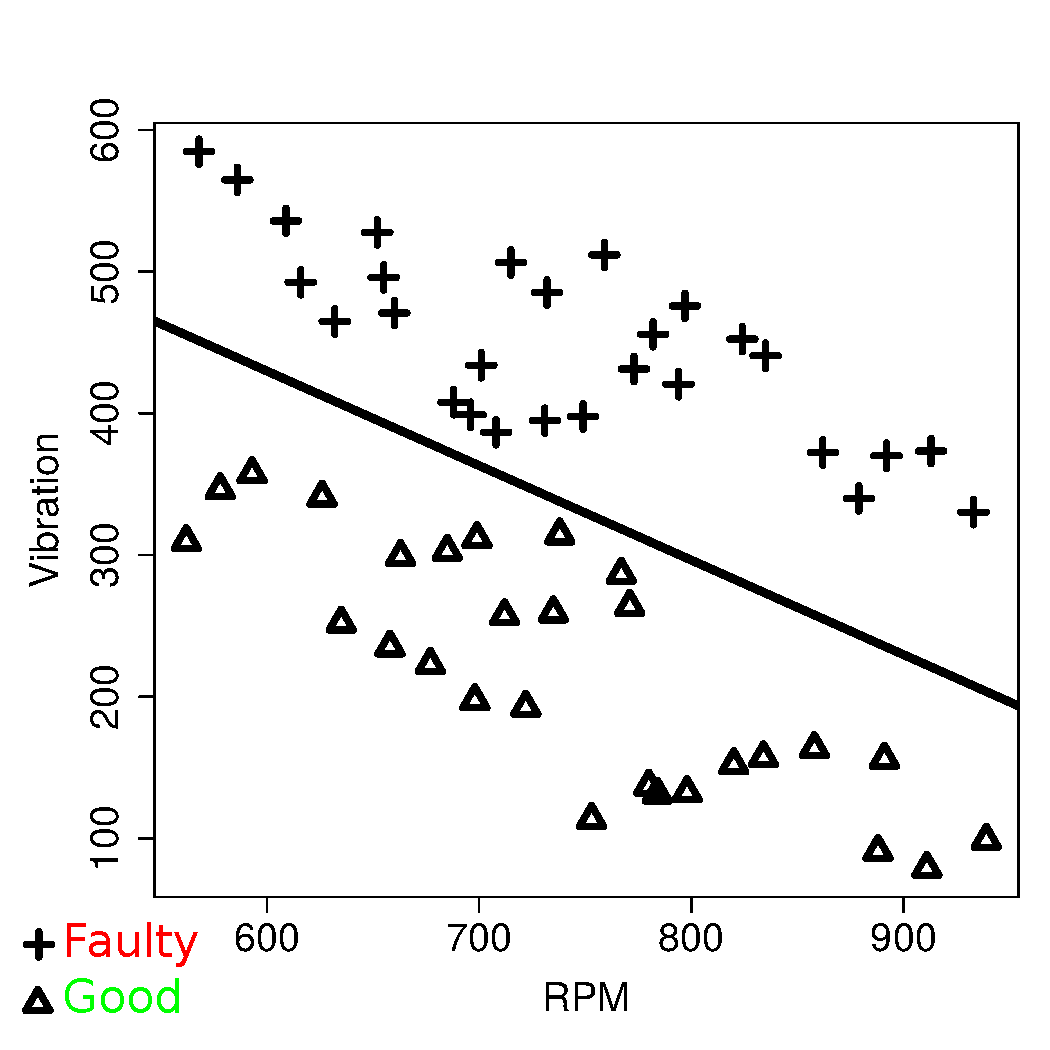
\includegraphics[scale=0.38]{fmlpda_figure_7_10_b}
	\end{center}
\end{frame}

\subsection{Classifiers and Problems}
\begin{frame}
  \frametitle{Classifiers and Problems}
    Linear classifier could not be sufficient (underfitting problem)
  	\begin{center}
	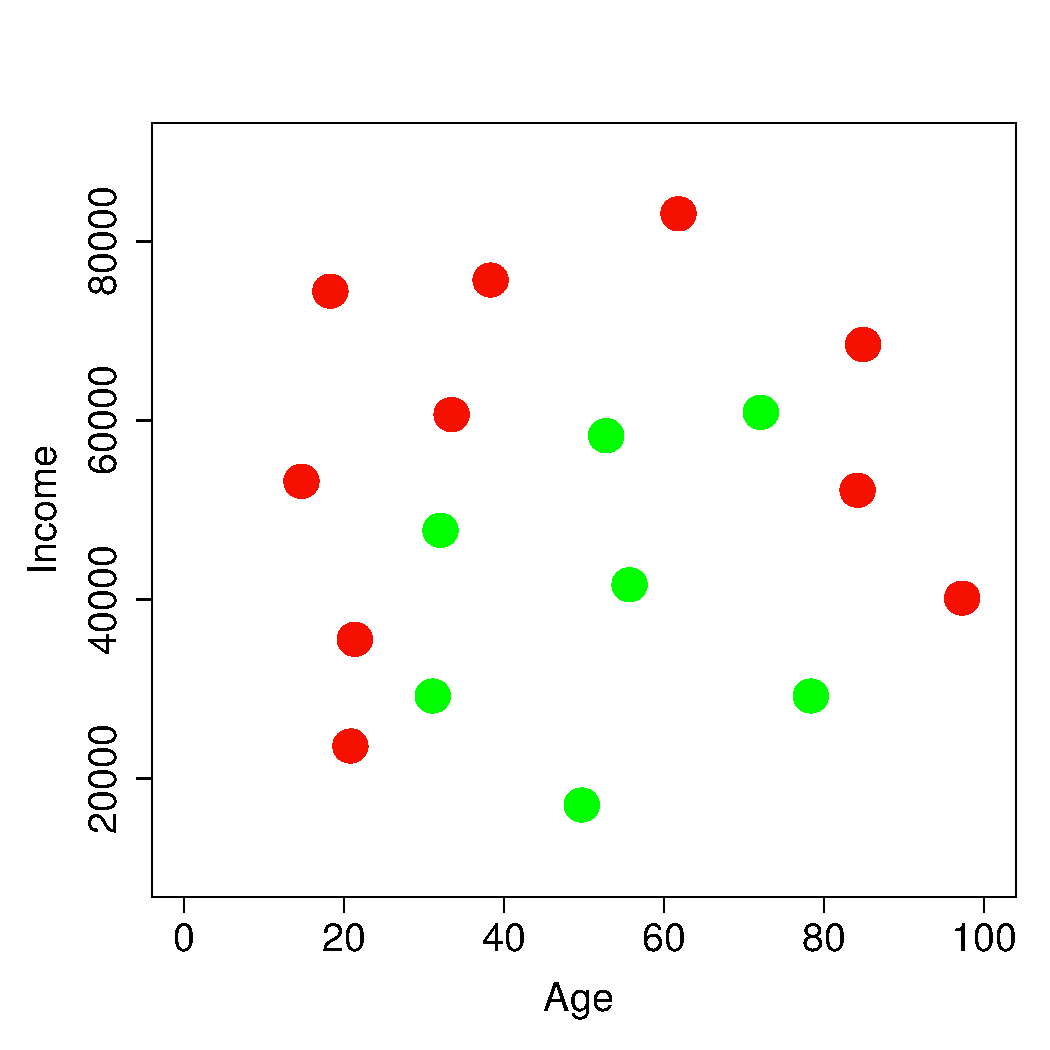
\includegraphics[scale=0.3]{fmlpda_figure_1_3_a}
	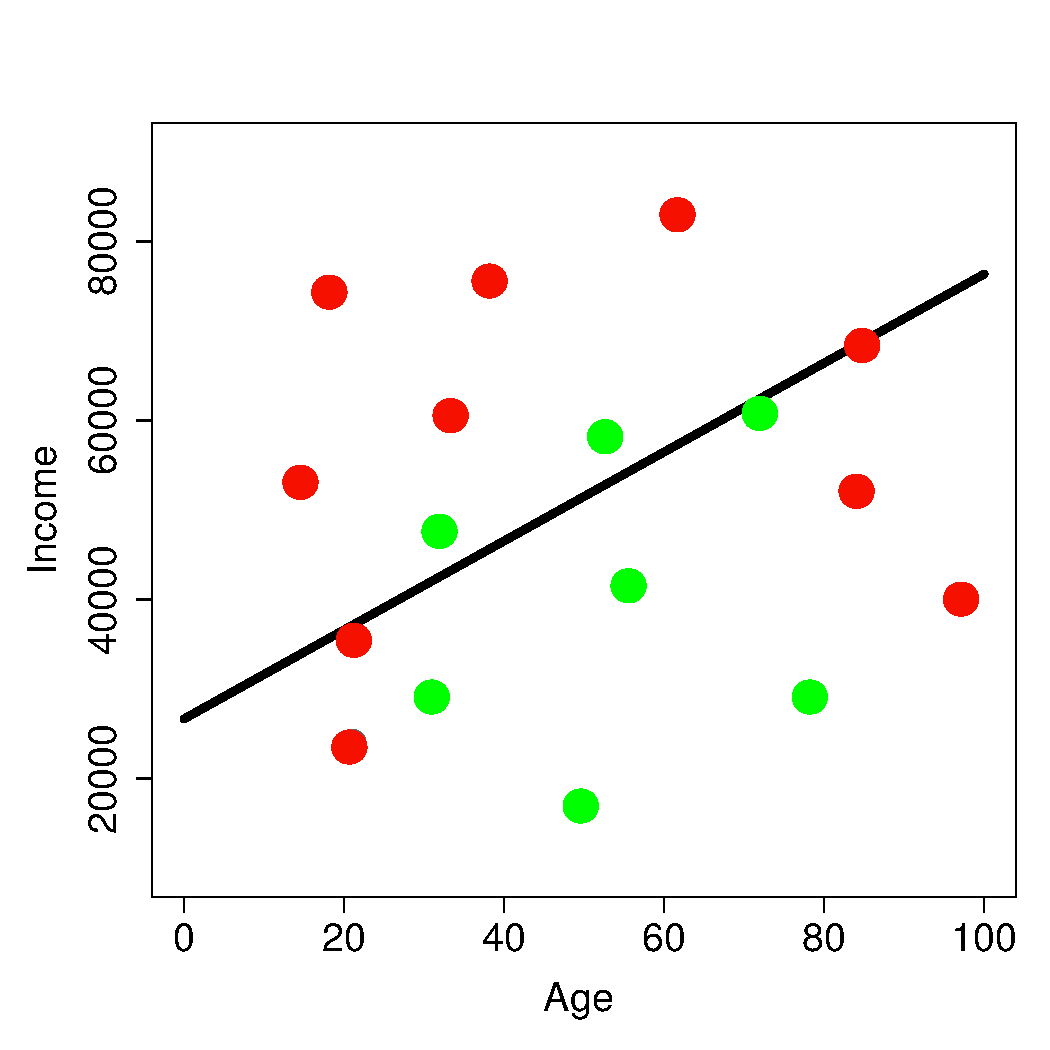
\includegraphics[scale=0.3]{fmlpda_figure_1_3_b}
	\end{center}
\end{frame}

\begin{frame}
  \frametitle{Classifiers and Problems}
    Also not linear classifier could not be sufficient (overfitting problem vs ``Just Right'' solution)
  	\begin{center}
	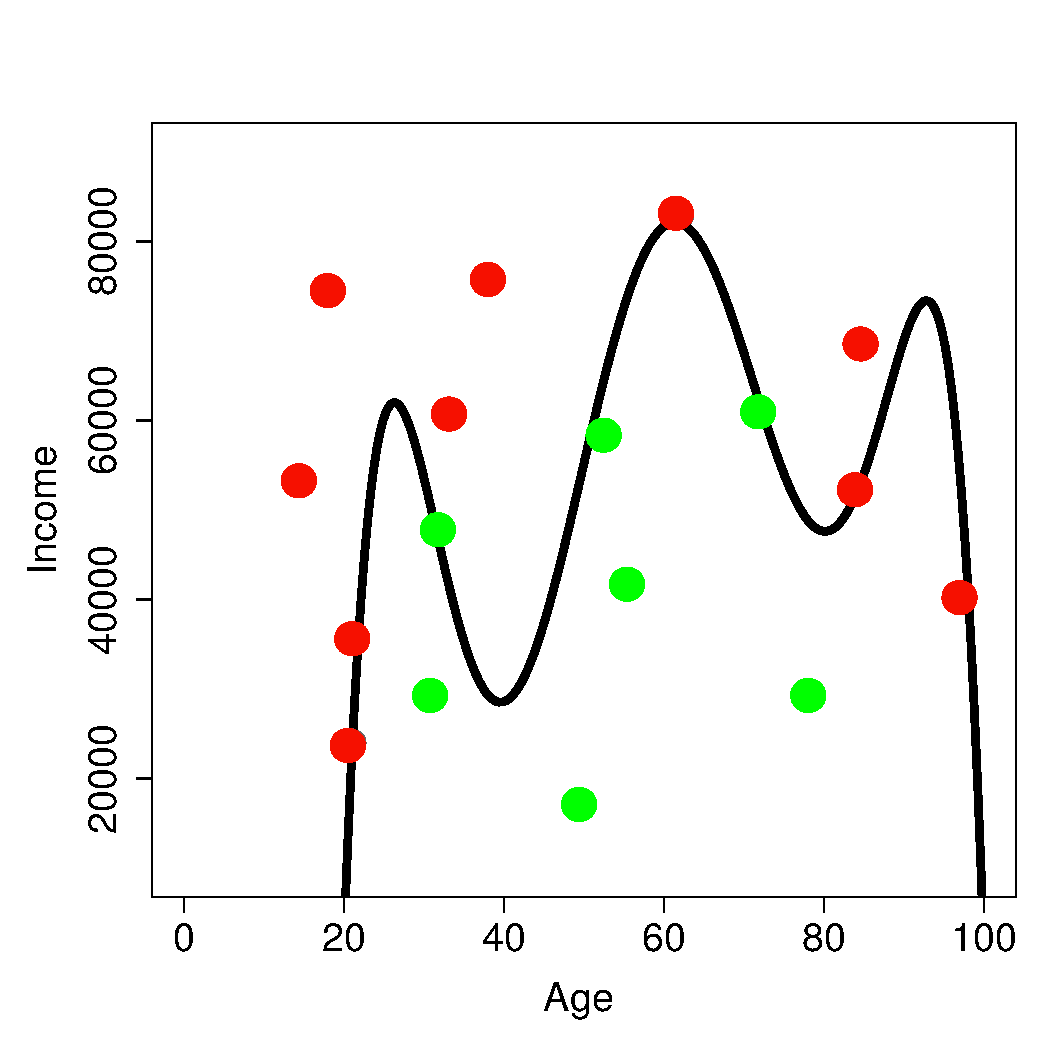
\includegraphics[scale=0.3]{fmlpda_figure_1_3_c}
	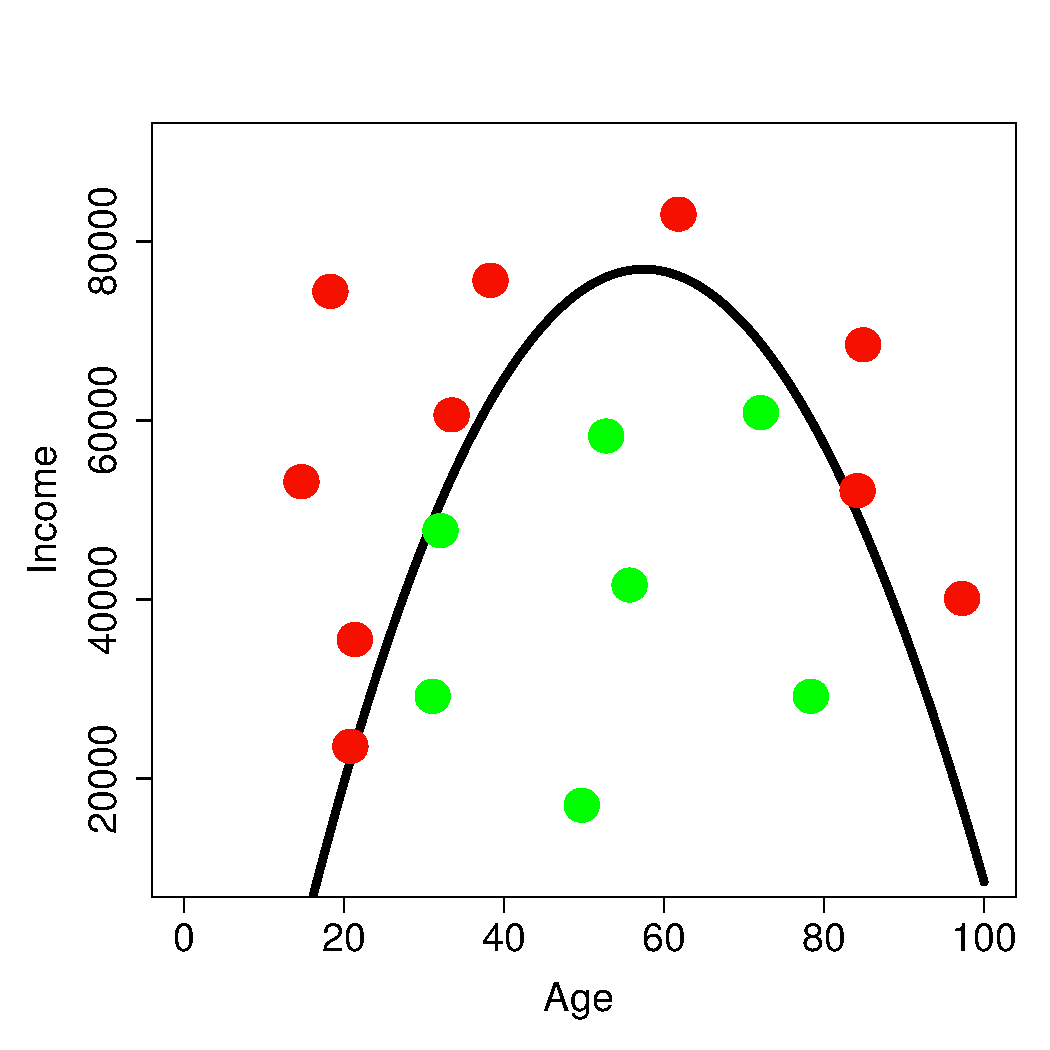
\includegraphics[scale=0.3]{fmlpda_figure_1_3_d}
	\end{center}
\end{frame}

\subsection{Feature Summary}
\begin{frame}
  \frametitle{Descriptive Features Summary}
    \begin{itemize}
	\item<+-> Can be continuous (e.g. number) or categorical (e.g. enumeration) 
	\item<+-> Can be considered as vectors
	\item<+-> Can be normalized (e.g. between [0,1], [-1,1], etc.)
	\item<+-> Can be also considered as probability (Bayesian approach)
	\item<+-> ...
   \end{itemize}
\end{frame}

\section{Fingerprint}
\subsection{Fingerprint Types}
\begin{frame}
  \frametitle{Fingerprint Types}
  \begin{itemize}
	\item<+-> \textbf{Browser:} we have an hash of the single browser a user usually use (Fingerprintjs2 acts in this way\footnotemark). 
	\item<+-> \textbf{Device:} (aka cross-browser) we have a device fingerprint identification. (using ever-cookie or other client side leverages could be a problem..)
	\item<+-> \textbf{User:} (aka cross-device) we have user fingerprint identification (tmx claims to do this)
   \end{itemize}
   \footnote[2]{ \href{https://valve.github.io/fingerprintjs2}{\url{https://valve.github.io/fingerprintjs2}} }
\end{frame}

\subsection{Fingerprint as Feature}
\begin{frame}
  \frametitle{Fingerprint as Feature}
  \begin{itemize}
	\item<+-> Fingerprints can be features!.. (\textbf{Browser} and \textbf{Device} types..)..
	\item<+-> \textbf{User} can be obtained using a mix of ML techniques + Expert Rules + other approaches (like graph databases, ...)
	\item<+-> In particular \textbf{User} could be obtained using a set of descriptive features that include \textbf{Browser} or \textbf{Device} and many more (ip, headers, os, etc..)
	\item<+-> Having a user hash could be very useful in tackling fraud...
	\item<+-> But could be also an over engineering approach.. perhaps we can obtain optimal results applying other (simpler) models on our existing data...
   \end{itemize}
\end{frame}


\section{Conclusion}
\subsection{What can we do?}
\begin{frame}
  \frametitle{What can we do?}
  \begin{itemize}
	\item<+-> Using ML is a natural fit in financial contexts... and we already use some technique...
	\item<+-> For example in Zip/City normalization we use a 1-Nearest-Neighbor simplified approach based on Jaro-Winkler distance..
	\item<+-> or we have developed Similarity library to match customer tuples (tune work need to made with logistic regression here...) 
   \end{itemize}
\end{frame}

\begin{frame}
  \frametitle{What can we do?}
  \begin{itemize}
	\item<+-> \textbf{Good News:} we have a lot of historical data..
	\item<+-> \textbf{Bad News:} they must be organized.. and this is hard(not impossible) due to data/architecture duplication/spread...
   \end{itemize}
\end{frame}

\begin{frame}
  \frametitle{What can we do? }
  \begin{itemize}
	\item<+-> Delegate to an external company could be a starting point...
	\item<+-> In any case we have to reorganize our data to have benefits all over the business.. and fraud detection would/will be a ``natural side effect''.. 
	\item<+-> We can use \textbf{expert rules} from arvato (our rules also!) and apply them to our data 
	\item<+-> We can obtain good results without using hyper-complex solutions.. for example fixing the ``ancient evil duplication menace'' of customer matching would be a good point in tackling fraud.. (e.g. using solr or similar solutions and detecting outliers over a returned distribution of results...) 
	\item<+-> Apply one of the ML approaches described above...
   \end{itemize}
\end{frame}


\section{References}
\subsection{list}
\begin{frame}
        \frametitle{Industry examples}
        \begin{itemize}
	\item \href{http://www.research.ibm.com/foiling-financial-fraud.shtml}{http://www.research.ibm.com/foiling-financial-fraud.shtml}
	\item \href{https://gizmodo.com/how-banks-use-machine-learning-to-know-a-crooks-using-y-1744771152}{https://gizmodo.com/how-banks-use-machine-learning-to-know-a-crooks-using-y-1744771152}
	\item \href{https://gigaom.com/2015/03/06/how-paypal-uses-deep-learning-and-detective-work-to-fight-fraud/}{https://gigaom.com/2015/03/06/how-paypal-uses-deep-learning-and-detective-work-to-fight-fraud/}
   \end{itemize}
\end{frame}


\begin{frame}
        \frametitle{References}
        \nocite{*}
        \bibliographystyle{alpha}
        \bibliography{bib_files/refs.bib}
\end{frame}

\end{document}
